\sectionthree{PDA Variants}
\begin{python0}
from solutions import *; clear()
\end{python0}

There are several variations on our definition of a PDA. 
It's not too difficult to prove that these definitions are equivalent to our 
definition.
The only exception is the last variant which is a
\textit{deterministic} PDA --
in the case of DFA, NFA are equal in power to DFA but
deterministic PDA is strictly weaker than PDA.

\newpage
\subsection{Emptying the stack}

Our acceptance condition for a string is based on state information.
Note that in our examples, we frequently also end our computation in an
accept state and the stack is empty.
In some books, acceptance means a computation lands in an accept state 
\textit{ and} the computation \textit{must also end in an empty stack}.
A PDA can easily be modified so that when a string is accepted, a computation
will land in an accept state with an empty stack.
How so?

You add a new state to your PDA, say we call it CLEAR, and you add
transition $(\ep, \ep \rightarrow \ep)$ from every accept state to CLEAR.
This allows the machine to enter CLEAR immediately.
Now add transitions from CLEAR to CLEAR that removes everything in the stack.
For instance if the set of stack symbols is $\{a, b, \$\}$, then you want to 
add transitions $(\ep, a \rightarrow \ep)$, $(\ep, b \rightarrow \ep)$,
and $(\ep, \$ \rightarrow \ep)$ from CLEAR to CLEAR.
Here's the picture where $q$ and $q'$ are accept states from the original PDA:

\begin{center}
\begin{tikzpicture}[shorten >=1pt,node distance=2cm,auto,initial text=]
\node[state,accepting] (q) at (0.0,0.0) {$q$};
\node[state,accepting] (q1) at (3.0,0.0) {$q'$};
\node[state] (c) at (1.5,-3.0) {CLEAR};

\path[->]
(c) edge [loop below] node {$(\ep,a\rightarrow\ep),(\ep,b\rightarrow\ep),(\ep,\$\rightarrow\ep)$} ()
(q) edge [left] node {$(\ep,\ep\rightarrow\ep)$} (c)
(q1) edge [right] node {$(\ep,\ep\rightarrow\ep)$} (c)

;
\end{tikzpicture}
\end{center}
    

At this point your PDA can accept or accept and clear the stack. 
To make sure that the stack \textit{ is} cleared when a string is accepted, you
just make the original accept states non--accepting:

\begin{center}
\begin{tikzpicture}[shorten >=1pt,node distance=2cm,auto,initial text=]
\node[state] (q) at (0.0,0.0) {$q$};
\node[state] (q1) at (3.0,0.0) {$q'$};
\node[state,accepting] (c) at (1.5,-3.0) {CLEAR};

\path[->]
(c) edge [loop below] node {$(\ep,a\rightarrow\ep),(\ep,b\rightarrow\ep),(\ep,\$\rightarrow\ep)$} ()
(q) edge [left] node {$(\ep,\ep\rightarrow\ep)$} (c)
(q1) edge [right] node {$(\ep,\ep\rightarrow\ep)$} (c)

;
\end{tikzpicture}
\end{center}


That's it!

Now all of this is well and dandy ... but the question is ... 
\textit{ why} would anyone want to empty the stack?

Well frequently you want to build a PDA by assemblying a bunch of PDAs
(you have already seen that for instance in DFAs/NFAs).
For instance, take a look at the construction of a PDA that accepts
the concatenation of the languages accepted by two given PDAs.
In that case, you want a second given PDA to use the stack.
So it would be good for the first given PDA to play nice by clearly
the stack.

\newpage
\subsection{Pushing a string}

Instead of pushing a character (or $\ep$) it's possible to define another 
type of PDA-like automata where everything is the same as our PDA except that 
you can 
push a string onto the stack.
In other words the transitions are of the form
\[
(a, b \rightarrow x)
\]
where $a \in \Sigma_\ep$, $b \in \Gamma_\ep$, and $x \in \Gamma^*$.
In \textit{ our} definition we require $x \in \Gamma_\ep = \Gamma \cup \{\ep\}$.
See the difference?
For instance such a PDA-like thingy can have a transition that looks like
this:
\[
(a, b \rightarrow aab)
\]
i.e. the input character read is $a$, and the top of the stack $b$ is
replaced by $aab$ (the $b$ goes into the stack first, followed by 
$a$, and then by another $a$).
Let's call such automatas PDA$_2$.
It seems that PDA$_2$s are more general and perhaps more powerful than our 
PDAs.

Well ... actually ... NO!

You can prove that if $P'$ is a PDA$_2$, then there is a PDA, $P$, such that
$L(P) = L(P')$ and vice versa.

Why? 
Obviously PDA$_2$ includes PDA since the definition of a PDA$_2$ is more
general.
But if you have a PDA$_2$ with the following transition
\[
q \xrightarrow{a, \, b \rightarrow c_1 \cdots c_n} p 
\]
where $c_i \in \Sigma$, you just modify the PDA$_2$ 
thingy by removing the above transition and adding the
following a corresponding 
series of transitions:
\[
q 
\xrightarrow{a, \, b \rightarrow c_1} q_1 
\xrightarrow{\ep, \, \ep \rightarrow c_2} q_2
\xrightarrow{\ep, \, \ep \rightarrow c_3}
\cdots  
\xrightarrow{\ep, \, \ep \rightarrow c_n} q_n 
\]
where the $q_i$ are new states.
In other words, you simply push one character at a time.
Then our PDA would accept the same language as the given PDA$_2$.



\newpage
\subsection{Initial stack state}

Because you almost always need to put a bottom-of-stack marker in a stack,
some definitions of a PDA actually allows one to specfy the initial contents
of the stack before executing the PDA.
In this case, the PDA is defined by $(Q, \Sigma, \Gamma, \delta, q_0, F, z)$
(it has an extra parameter), where $z \in \Gamma^*$ is the initial contents
on the stack.
So in this case where you need a bottom-of-stack marker, you could have 
started off with a PDA of the form $(Q, \Sigma, \Gamma, \delta, q_0, F, \$)$
and not bother to push the \$ onto the stack as a first transition.

All the above are variants of our PDA definition.
Remember that they are all equal in power to our usual PDA:
The language accepted by one PDA variant is also accepted by another variant.

%-*-latex-*-

\begin{ex} 
  \label{ex:prob-00}
  \tinysidebar{\debug{exercises/{disc-prob-28/question.tex}}}

  \solutionlink{sol:prob-00}
  \qed
\end{ex} 
\begin{python0}
from solutions import *
add(label="ex:prob-00",
    srcfilename='exercises/discrete-probability/prob-00/answer.tex') 
\end{python0}


\newpage
\subsection{Null stack acceptance}

We've defined acceptance as accept a string when the computation ends in an
accept state.

There's another definition of acceptance where a string is accepted when the 
computation ends with an empty stack. 
In this case, you need not end in an accept state.
(In fact for such automatas, there is no concept of accept state.)
This is called \defterm{acceptance by null stack}.
Usually to indicate this type of acceptance, I would write $N(P)$
instead of $L(P)$ where $P$ is a PDA of this type.
Again you do not get new languages by using this definition of acceptance.


[PREVIOUS
VERSION: 
In other books, acceptance means the PDA must reach the accept state
\textit{ and} the stack must be empty.
All these definitions of acceptance are actually equivalent to ours
in the sense that you can restructure your PDA to conform to another definition
of acceptance without any problem (or pain).]


Here's how you convert a regular PDA $P$ to another $P'$ so that the 
$L(P) = N(P')$.
First you simply clear the stack after accepting a string (see above on how to
do that.)
Is that enough?
NO! According to the original definition of acceptance for $P$,
a string is accepted only when there is a computation that lands in an accept 
state -- it's possible that during this computation the stack is empty.
So the first thing we need to do is in fact to ensure the $P$ can never
have an empty stack.
So we pick a special symbol, say \#, and push \# onto the stack before even
running $P$. Now add to the state that clears the stack the transition
to clear \# as well.
So the picture looks like this where $s$ is the start state of $P$ and,
say $q$ and $q'$ are accept states of $P$, and $P'$ is the new PDA:

\begin{samepage}
\begin{verbatim}
P'
+--------------------------------------------------+
|                        P                         |
|                       +-------------------+      |
|             e, e->#   |                   |      |
| -> (START) ------------> (s)     (q) (q') |      |
|                       |           |   |   |      |
|                       +-----------|---|---+      |
|                          (e, e->e)|   |(e, e->e) |
|                                   v   v          |
|                                  (CLEAR)         |
|                                   |   ^          |
|                                   |   |          |
|                                   +---+          |
|                                 (e, a->e)        |
|                                 (e, b->e)        |
|                                 (e, #->e)        |
+--------------------------------------------------+
\end{verbatim}
\end{samepage}

In this example, I'm assuming that the set of stack symbols of $P$ is
$\{a, b\}$.
In general at state CLEAR you have to clear all the symbols in the stack
symbols of $P$ from the stack and the new symbol \#.
Of course for this new PDA we do not need to make CLEAR an accept state since
acceptance is defined in terms of the stack being empty, i.e. we're
interested in $N(P')$ and not $L(P')$.
In fact you can even keep $q$ and $q'$ as accept states too.

One final thing (and I hope you already realized this): 
Notice that at START, the stack \textit{ is} empty.
This means that the empty string is accepted regardless of the PDA (of this
type)!
So if you want to use acceptance by null stack and the language accepted
does not contain $\ep$, you can declare that your PDA already has \# as the 
initial stack content.

\begin{samepage}
\begin{verbatim}
P' (initial stack is #)
+--------------------------------------------------+
|                        P                         |
|                       +-------------------+      |
|                       |                   |      |
| -----------------------> (s)     (q) (q') |      |
|                       |           |   |   |      |
|                       +-----------|---|---+      |
|                          (e, e->e)|   |(e, e->e) |
|                                   v   v          |
|                                  (CLEAR)         |
|                                   |   ^          |
|                                   |   |          |
|                                   +---+          |
|                                 (e, a->e)        |
|                                 (e, b->e)        |
|                                 (e, #->e)        |
+--------------------------------------------------+
\end{verbatim}
\end{samepage}

From now on we will move freely between the different variants of the PDA.

%-*-latex-*-

\begin{ex} 
  \label{ex:prob-00}
  \tinysidebar{\debug{exercises/{disc-prob-28/question.tex}}}

  \solutionlink{sol:prob-00}
  \qed
\end{ex} 
\begin{python0}
from solutions import *
add(label="ex:prob-00",
    srcfilename='exercises/discrete-probability/prob-00/answer.tex') 
\end{python0}


\newpage
\subsection{Deterministic PDA (DPDA)}

One \textit{ final} variant:
Note that our PDAs are nondeterministic.
You can define a deterministic PDA (DPDA).
(You should be able to guess what a DPDA looks like by now, right?)

These are actually \textit{ not} equal in power to PDAs.

In other words there are languages accepted by a PDA that is not accepted
by any DPDA.
Later we will show that PDA languages are the same as CFL and they include
regular; DPDA languages are in between.
In other words, regular languages are included in DPDA languages and DPDA
languages are included in CFLs.
Languages accepted by DPDA are said to be DCFL (deterministic CFL).

The reason for DPDA is because of parsing:
CFL can be amgiuous and parsing is slow (CYK has a runtime of $O(n^3)$).
DCFL are not ambiguous and runtime parsing is $O(n)$.
In particular, DCFL are important in compilers for programming languages.
We won't talk about these anymore.
(See compiler notes.)

\begin{center}
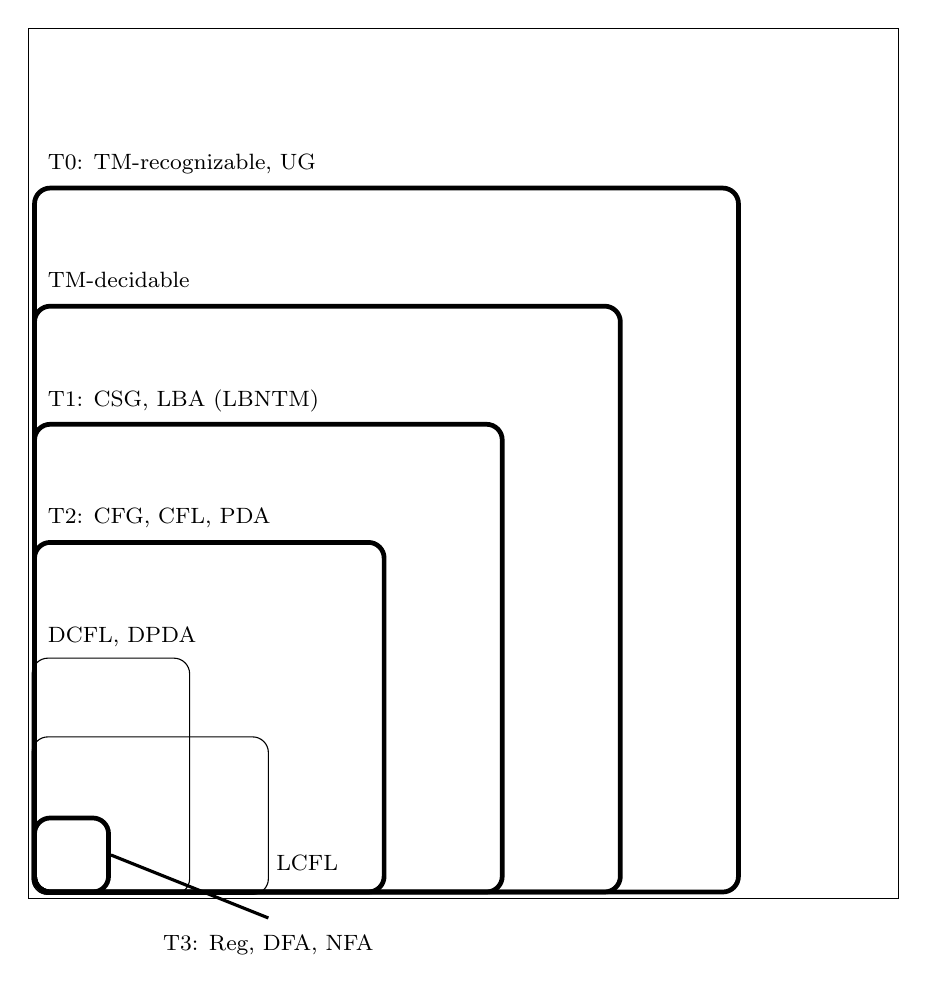
\begin{tikzpicture}

\draw (5.475, 5.475)
  node[draw, , , color=black,
       rounded corners=0cm, inner sep=0cm] {

\begin{minipage}[t][11.05cm]{11.05cm}
\mbox{}

\end{minipage}

};
\draw (0.5, 0.5)
  node[draw, line width=0.06cm, , color=black,
       rounded corners=0.2cm, inner sep=0cm] {

\begin{minipage}[t][0.94cm]{0.94cm}
\mbox{}

\end{minipage}

};
\draw (3.0, -0.65)
  node[draw=none, line width=0cm, , color=black,
       rounded corners=0cm, inner sep=0cm] {

\begin{minipage}[t][0.7cm]{2cm}
\mbox{}

\end{minipage}

};\draw (3.0, -0.65) node[color=black] {{\footnotesize T3: Reg, DFA, NFA}};\draw[line width=0.04cm,black] (1,0.5) to  (3.0,-0.3);

\draw (1.0, 1.5)
  node[draw, , , color=black,
       rounded corners=0.2cm, inner sep=0cm] {

\begin{minipage}[t][3.0cm]{2.0cm}
\mbox{}

\end{minipage}

};
\draw (2.6, 3.3)
  node[draw=none, line width=0cm, , color=black,
       rounded corners=0cm, inner sep=0cm] {

\begin{minipage}[t][0.1cm]{4.8cm}
\mbox{}

\end{minipage}

};
\draw (2.6, 3.3) node[color=black,
 inner sep=0cm] {
 
\begin{minipage}[t][0.1cm]{4.8cm}
{\footnotesize DCFL, DPDA}
\end{minipage}

};
\draw (1.5, 1.0)
  node[draw, , , color=black,
       rounded corners=0.2cm, inner sep=0cm] {

\begin{minipage}[t][2.0cm]{3.0cm}
\mbox{}

\end{minipage}

};
\draw (4.1, 0.4)
  node[draw=none, line width=0cm, , color=black,
       rounded corners=0cm, inner sep=0cm] {

\begin{minipage}[t][0.1cm]{2.0cm}
\mbox{}

\end{minipage}

};
\draw (4.1, 0.4) node[color=black,
 inner sep=0cm] {
 
\begin{minipage}[t][0.1cm]{2.0cm}
{\footnotesize LCFL}
\end{minipage}

};
\draw (2.25, 2.25)
  node[draw, line width=0.06cm, , color=black,
       rounded corners=0.2cm, inner sep=0cm] {

\begin{minipage}[t][4.44cm]{4.44cm}
\mbox{}

\end{minipage}

};
\draw (2.85, 4.8)
  node[draw=none, line width=0cm, , color=black,
       rounded corners=0cm, inner sep=0cm] {

\begin{minipage}[t][0.1cm]{5.3cm}
\mbox{}

\end{minipage}

};
\draw (2.85, 4.8) node[color=black,
 inner sep=0cm] {
 
\begin{minipage}[t][0.1cm]{5.3cm}
{\footnotesize T2: CFG, CFL, PDA}
\end{minipage}

};
\draw (3.0, 3.0)
  node[draw, line width=0.06cm, , color=black,
       rounded corners=0.2cm, inner sep=0cm] {

\begin{minipage}[t][5.94cm]{5.94cm}
\mbox{}

\end{minipage}

};
\draw (2.85, 6.3)
  node[draw=none, line width=0cm, , color=black,
       rounded corners=0cm, inner sep=0cm] {

\begin{minipage}[t][0.1cm]{5.3cm}
\mbox{}

\end{minipage}

};
\draw (2.85, 6.3) node[color=black,
 inner sep=0cm] {
 
\begin{minipage}[t][0.1cm]{5.3cm}
{\footnotesize T1: CSG, LBA (LBNTM)}
\end{minipage}

};
\draw (3.75, 3.75)
  node[draw, line width=0.06cm, , color=black,
       rounded corners=0.2cm, inner sep=0cm] {

\begin{minipage}[t][7.44cm]{7.44cm}
\mbox{}

\end{minipage}

};
\draw (2.85, 7.8)
  node[draw=none, line width=0cm, , color=black,
       rounded corners=0cm, inner sep=0cm] {

\begin{minipage}[t][0.1cm]{5.3cm}
\mbox{}

\end{minipage}

};
\draw (2.85, 7.8) node[color=black,
 inner sep=0cm] {
 
\begin{minipage}[t][0.1cm]{5.3cm}
{\footnotesize TM-decidable}
\end{minipage}

};
\draw (4.5, 4.5)
  node[draw, line width=0.06cm, , color=black,
       rounded corners=0.2cm, inner sep=0cm] {

\begin{minipage}[t][8.94cm]{8.94cm}
\mbox{}

\end{minipage}

};
\draw (2.85, 9.3)
  node[draw=none, line width=0cm, , color=black,
       rounded corners=0cm, inner sep=0cm] {

\begin{minipage}[t][0.1cm]{5.3cm}
\mbox{}

\end{minipage}

};
\draw (2.85, 9.3) node[color=black,
 inner sep=0cm] {
 
\begin{minipage}[t][0.1cm]{5.3cm}
{\footnotesize T0: TM-recognizable, UG}
\end{minipage}

};
\end{tikzpicture}

\end{center}


